\section{最初の節}

私はその人\citep{Asakura2021}を常に先生と呼んでいた.
だからここでもただ先生と書くだけで本名は打ち明けない.
これは世間を憚かる遠慮というよりも,その方が私にとって自然だからである.
私はその人の記憶を呼び起すごとに,すぐ「先生」といいたくなる.
筆を執っても心持は同じ事である.
よそよそしい頭文字などはとても使う気にならない.

まるで\figref{fig:HolweckPump}に示すネジ溝ポンプのように.
\pgref{eq:Boltzmann}にBoltzmann方程式を示す.

\begin{figure}[b]
  \centering
  \begin{minipage}{0.6\hsize}
    \centering
    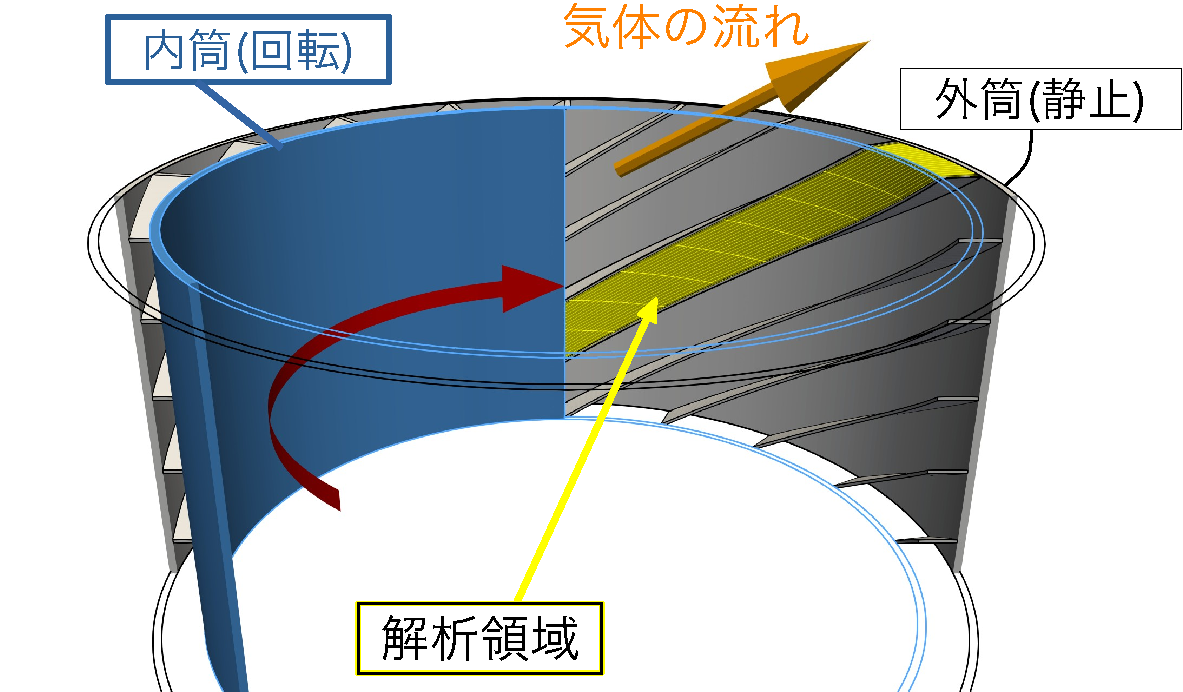
\includegraphics[width=0.7\hsize]{HolweckPump.pdf}
    \figcaption{ネジ溝ポンプのモデル図.}
    \label{fig:HolweckPump}
  \end{minipage}
  \begin{minipage}{0.3\hsize}
    \centering
    \tblcaption{排他的論理和}
    \begin{tabular}{cc|c}
      $X$ & $Y$ & $X \mathrm{xor} Y$ \\\hline
      0 & 0 & 0 \\
      1 & 0 & 1 \\
      0 & 1 & 1 \\
      1 & 1 & 0 \\
    \end{tabular}
  \end{minipage}
  
\end{figure}

